\subsection{Appendix A: Source code} \label{appendixA}
The code used for this project is available at \url{https://github.com/GauteJ1/FYS-STK-projects}. Instructions for running the code are located in \texttt{ project\_1/README.md}. All plots and results in this paper are easily reproducible in the Jupyter notebook files in this repository, by following the instructions mentioned above.

\subsection{Appendix B: Pen and paper calculations}\label{appendixB}

In this section, the calculations for some of our theretical expressions are presented. 

\begin{align}\label{a1}
    \fv{y_i} & = \fv{\sum_j x_{ij}\beta_j + \epsilon_i} \nonumber \\
    & = \fv{\sum_j x_{ij}\beta_j} + \fv{\epsilon_i} \nonumber \\ 
    & = \sum_j x_{ij}\beta_j + 0 \nonumber \\
    & = \mathbf{X}_{i,*}\boldsymbol{\beta}
\end{align}

Eq. \ref{a1}: Calculation of the expectation value of the true $y_i$, using the assumption that $\fv{\epsilon_i} = 0$. 



\begin{align}\label{a2}
    \text{var}(y_i) & = \fv{(y_i -\fv{y_i})^2} \nonumber \\
    & = \fv{y_i^2} - \fv{y_i}^2 \nonumber \\ 
    & = \fv{(\sum_j x_{ij}\beta_j + \epsilon_i)^2} - \fv{y_i}^2 \nonumber \\
    & = \fv{(\sum_j x_{ij}\beta_j)^2} + \fv{\epsilon_i^2} + 2\fv{\sum_j x_{ij}\beta_j \epsilon_i } - \fv{y_i}^2 \nonumber \\
    & = \fv{y_i}^2 + \fv{\epsilon_i^2} + 2\fv{y_i}^2\cdot 0 - \fv{y_i}^2 \nonumber \\ 
    & = \sigma^2
\end{align}

Eq. \ref{a2}: Calculation of the variance of the true $y_i$. Here $\fv{\epsilon_i} = 0$ and $\fv{\epsilon_i^2} = \text{var}(\boldsymbol{\epsilon}) = \sigma^2$, as $\epsilon \sim  
\mathcal{N}(0,\sigma^2)$.

\begin{align}\label{a3}
    \fv{\hat{\bet}} & = \fv{(\mathbf{X}^T\mathbf{X})^{-1}\mathbf{X}^T \y} \nonumber \\ 
    & = (\mathbf{X}^T\mathbf{X})^{-1}\mathbf{X}^T \fv{\y} \nonumber \\ 
    & = (\mathbf{X}^T\mathbf{X})^{-1}\mathbf{X}^T \mathbf{X}\bet \nonumber \\
    & = \unit \bet \nonumber \\
    & = \bet 
\end{align}

Eq. \ref{a3}: Calculation of the bias for the OLS estimator $\hat{\bet}$. The result from Eq. \ref{a1} is used going from the second to the third line.

\begin{align}\label{a4}
    \text{var}(\hat{\bet}) & = \fv{(\hat{\bet}-\fv{\hat{\bet}})^2} \nonumber \\
    & = \fv{(\hat{\bet}-\fv{\hat{\bet}})(\hat{\bet}-\fv{\hat{\bet}})^T} \nonumber \\ 
    & = \fv{(\hat{\bet}-\bet)(\hat{\bet}-\bet)^T} \nonumber \\ 
    & = \fv{(\hat{\bet}-\bet)(\hat{\bet}^T-\bet^T)} \nonumber \\
    & = \fv{\hat{\bet}\hat{\bet}^T} - \fv{\hat{\bet}\bet^T} - \fv{\bet \hat{\bet}^T} + \fv{\bet \bet^T} \nonumber \\
    & = \fv{\hat{\bet}\hat{\bet}^T} - \bet\bet^T - \bet\bet^T + \bet\bet^T \nonumber \\
    & = \fv{\hat{\bet}\hat{\bet}^T} - \bet\bet^T \nonumber \\
    & = \fv{\betta(\betta)^T} - \bet\bet^T \nonumber \\
    & = \fv{\betta \y^T \mathbf{X}(\mathbf{X}^T\mathbf{X})^{-T}} - \bet\bet^T \nonumber \\
    & = (\mathbf{X}^T\mathbf{X})^{-1}\mathbf{X}^T\fv{\y\y^T}\mathbf{X}(\mathbf{X}^T\mathbf{X})^{-T} - \bet\bet^T \nonumber \\
    & = (\mathbf{X}^T\mathbf{X})^{-1}\mathbf{X}^T(\mathbf{X}\bet \bet^T \mathbf{X}^T \\ 
    & \quad + \fv{\boldsymbol{\epsilon}^2})\mathbf{X}(\mathbf{X}^T\mathbf{X})^{-T} - \bet\bet^T \nonumber \\
    & = \bet \bet^T + \sigma^2 (\mathbf{X}^T\mathbf{X})^{-1} - \bet \bet^T \nonumber \\
    & = \sigma^2 (\mathbf{X}^T\mathbf{X})^{-1}
\end{align}

Eq. \ref{a4}: Calculation of the variance of the ordinary least squares estimator. \mia{smt else?}

\begin{align}\label{a5}
    \fv{(\mathbf{y}-\yt)^2} & = \fv{(\mathbf{y} - \fv{\yt} + \fv{\yt} -\yt)^2} \nonumber \\
    & = \fv{(\mathbf{y} - \fv{\yt})^2} + \fv{(\fv{\yt} -\yt)^2} \nonumber \\
    & \;\;\;\; + 2\fv{(\mathbf{y} - \fv{\yt})(\fv{\yt} -\yt)} \nonumber \\
    & = \fv{(\mathbf{f} + \boldsymbol{\epsilon} - \fv{\yt})^2} + \fv{(\yt - \fv{\yt})^2} \nonumber \\
    & = \fv{(\mathbf{f}-\fv{\yt})^2}+\fv{\boldsymbol{\epsilon}^2} \nonumber \\
    & \;\;\;\; + 2\fv{(\mathbf{f}-\fv{\yt})\boldsymbol{\epsilon}} + \fv{(\yt - \fv{\yt})^2}  \nonumber \\
    & = \fv{(\mathbf{f}-\fv{\yt})^2} + \fv{(\yt - \fv{\yt})^2} +\fv{\boldsymbol{\epsilon}^2}\nonumber \\
    & = \text{Bias}(\yt)^2 + \text{var}(\yt) + \sigma^2
\end{align}

Eq. \ref{a5}: Decomposition of the expected loss in terms of bias and variance. As $\bold{f}$ is unknown, $\y$ is used in calculations. 

% In the calculations these terms are zero: 

% \begin{align*}
%     2\fv{(\mathbf{y} - \fv{\yt})(\fv{\yt} -\yt)} & = 2\fv{\mathbf{y} - \fv{\yt}}\fv{\fv{\yt} -\yt} \nonumber \\ 
%     & = 2\fv{\mathbf{y} - \fv{\yt}} (\fv{\yt}-\fv{\yt}) \nonumber \\ 
%     & = 2\fv{\mathbf{y} - \fv{\yt}} \cdot 0 \nonumber \\
%     & = 0
% \end{align*}

% \begin{align*}
%     2\fv{(\mathbf{f}-\fv{\yt})\boldsymbol{\epsilon}} & =  2 \fv{(\mathbf{f}-\fv{\yt})}\fv{\boldsymbol{\epsilon}} \nonumber \\
%     & = 2 \fv{(\mathbf{f}-\fv{\yt})} \cdot 0 \nonumber \\
%     & = 0
% \end{align*}

% Have also used: 

% \begin{align*}
%     \fv{\boldsymbol{\epsilon}} & = 0 \nonumber \\
%     \fv{\boldsymbol{\epsilon}^2} & = \text{var}(\boldsymbol{\epsilon}) = \sigma^2 \nonumber \\
% \end{align*}

\subsection{Appendix C: Use of AI} \label{appendixC}

\mia{State use of AI}


\gaute{clearpage here if needed}


\subsection{Appendix D: Plots not included in the report} \label{appendixD}

\begin{figure}
    \centering
    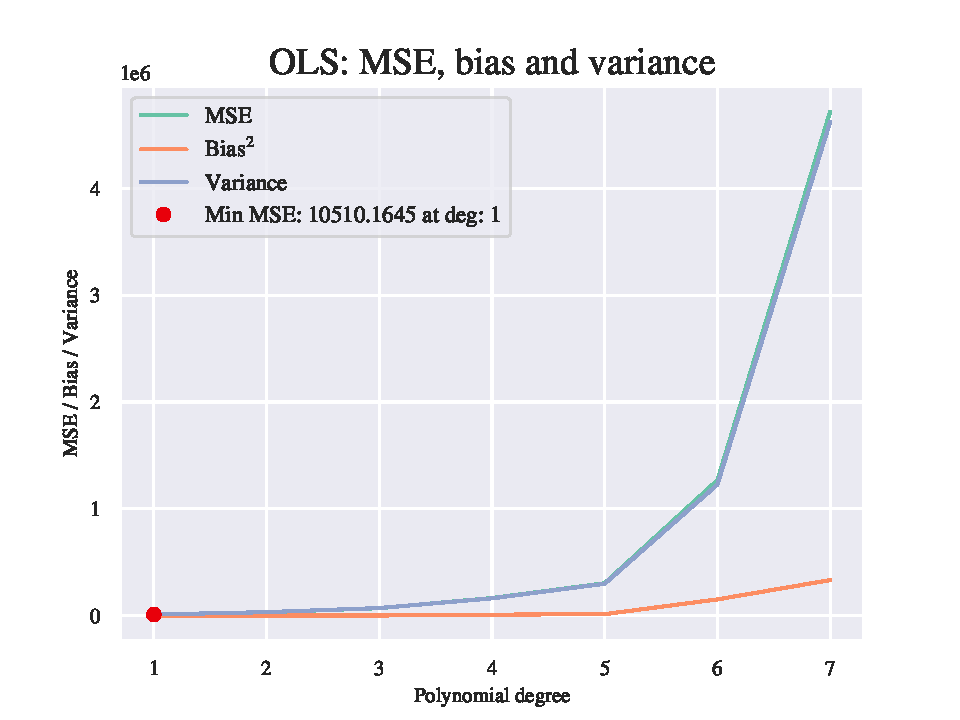
\includegraphics[width=1\linewidth]{project_1/figures/figures_in_appendix/bias_var_terrain_bootstrap.pdf}
    \caption{Caption}
    \label{fig:ref}
\end{figure}

\begin{figure}
    \centering
    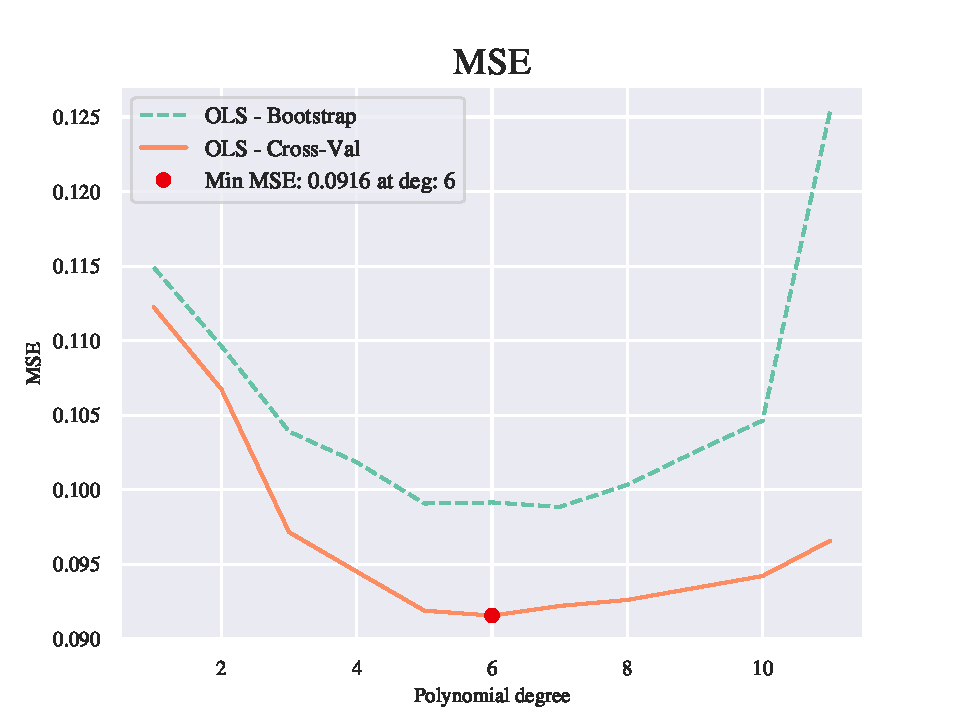
\includegraphics[width=1\linewidth]{project_1/figures/figures_in_appendix/CV_BS_OLS_Franke_Noise.pdf}
    \caption{Caption}
    \label{fig:ref}
\end{figure}

\begin{figure}
    \centering
    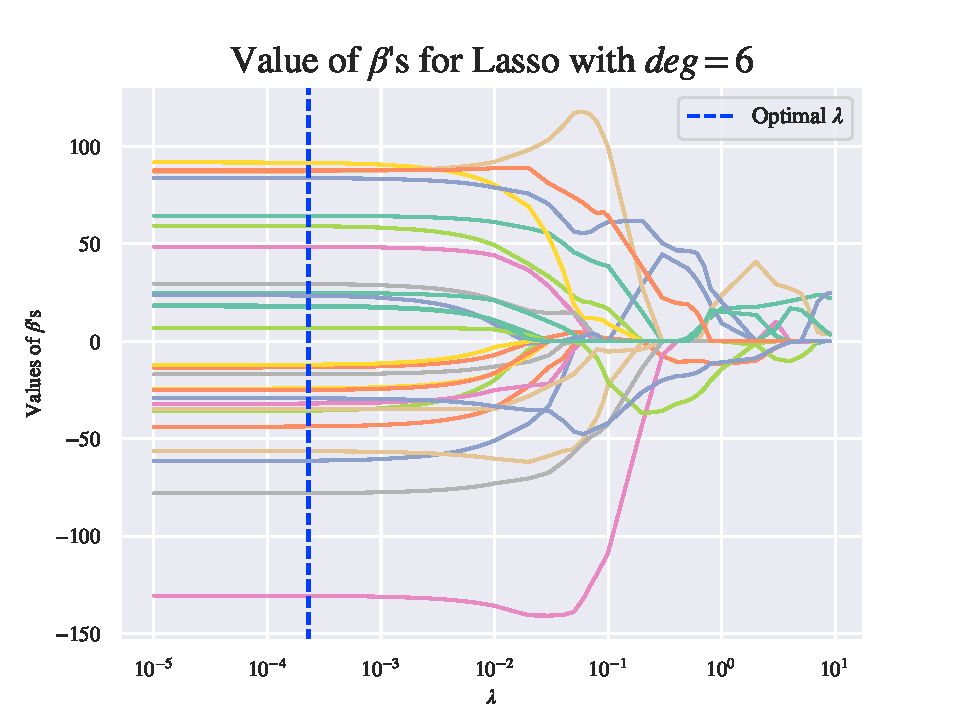
\includegraphics[width=1\linewidth]{project_1/figures/figures_in_appendix/Lasso_Betas_lambda_terrain_const_deg.pdf}
    \caption{Caption}
    \label{fig:ref}
\end{figure}

\begin{figure}
    \centering
    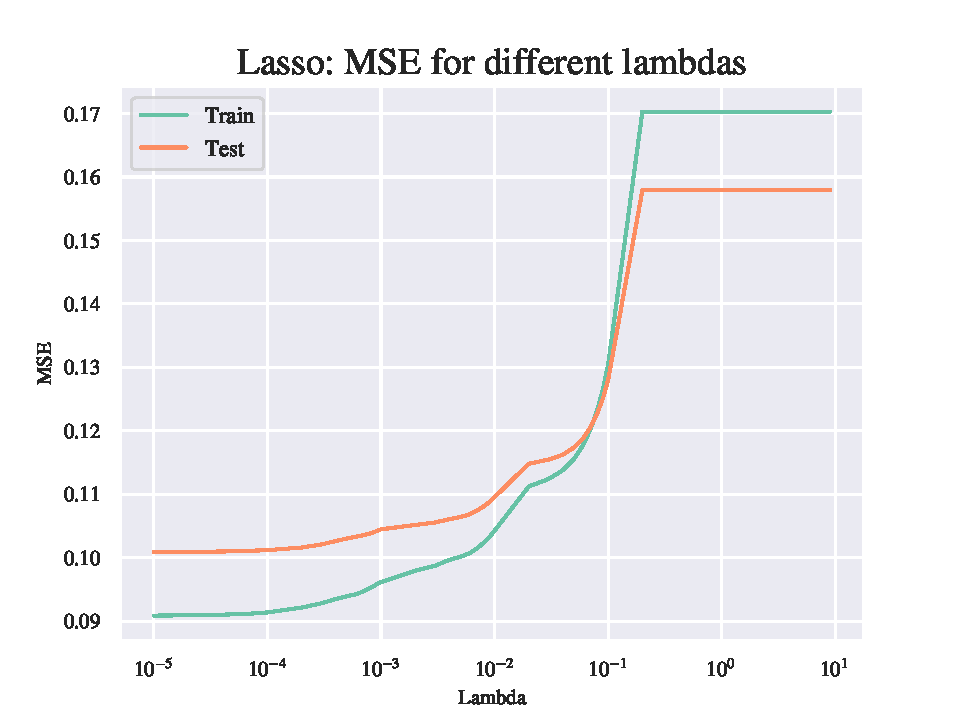
\includegraphics[width=1\linewidth]{project_1/figures/figures_in_appendix/Lasso_MSE_Franke_Noise.pdf}
    \caption{Caption}
    \label{fig:ref}
\end{figure}

\begin{figure}
    \centering
    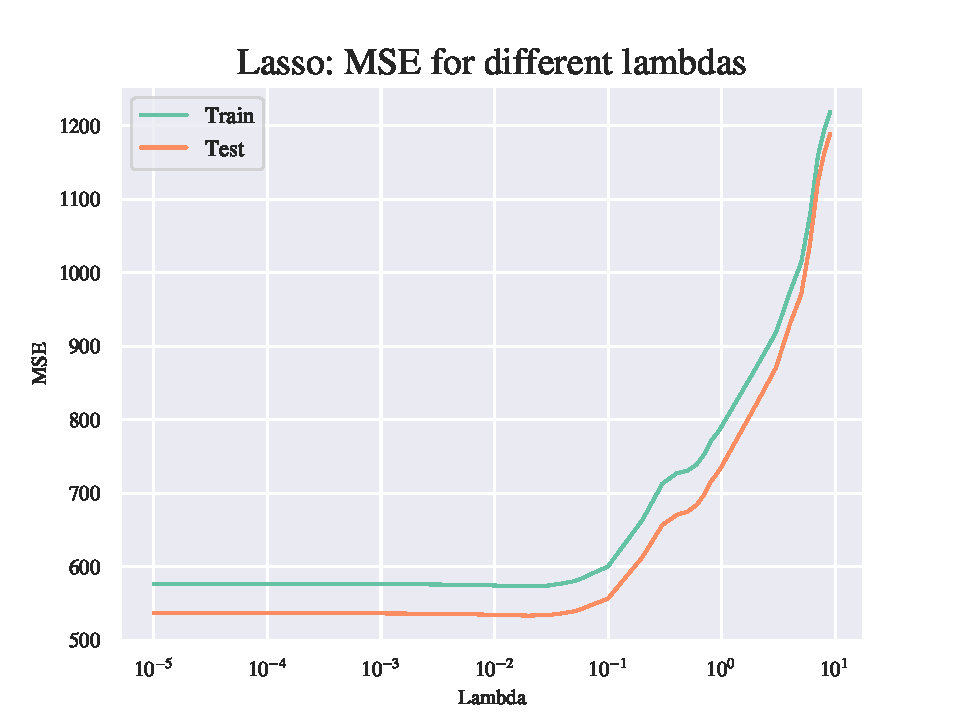
\includegraphics[width=1\linewidth]{project_1/figures/figures_in_appendix/Lasso_MSE_terrain.pdf}
    \caption{Caption}
    \label{fig:ref}
\end{figure}

\begin{figure}
    \centering
    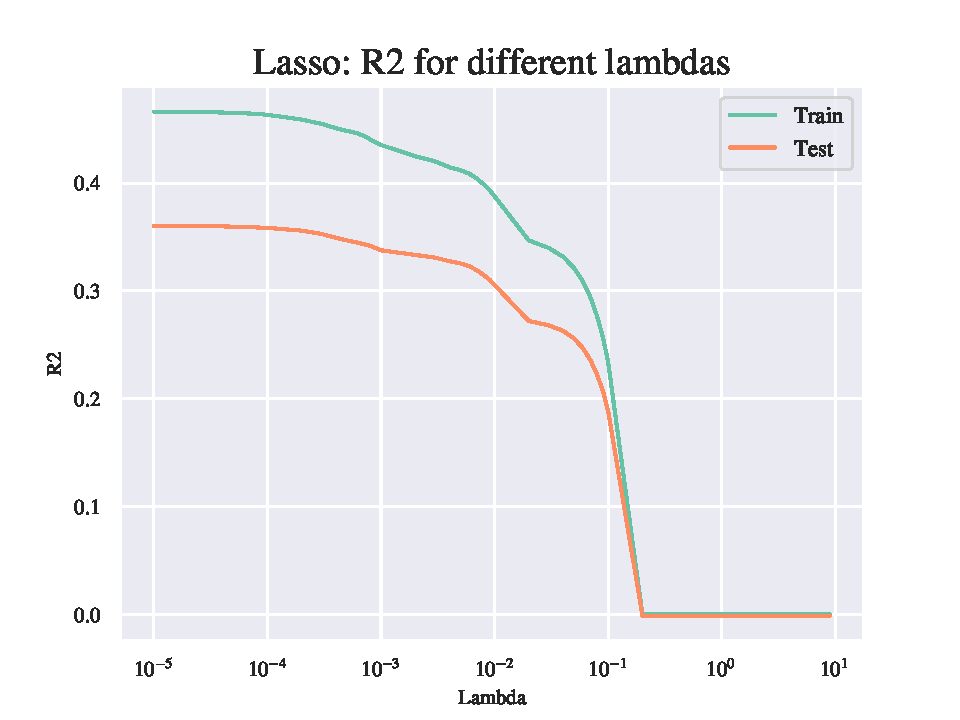
\includegraphics[width=1\linewidth]{project_1/figures/figures_in_appendix/Lasso_R2_Franke_Noise.pdf}
    \caption{Caption}
    \label{fig:ref}
\end{figure}

\begin{figure}
    \centering
    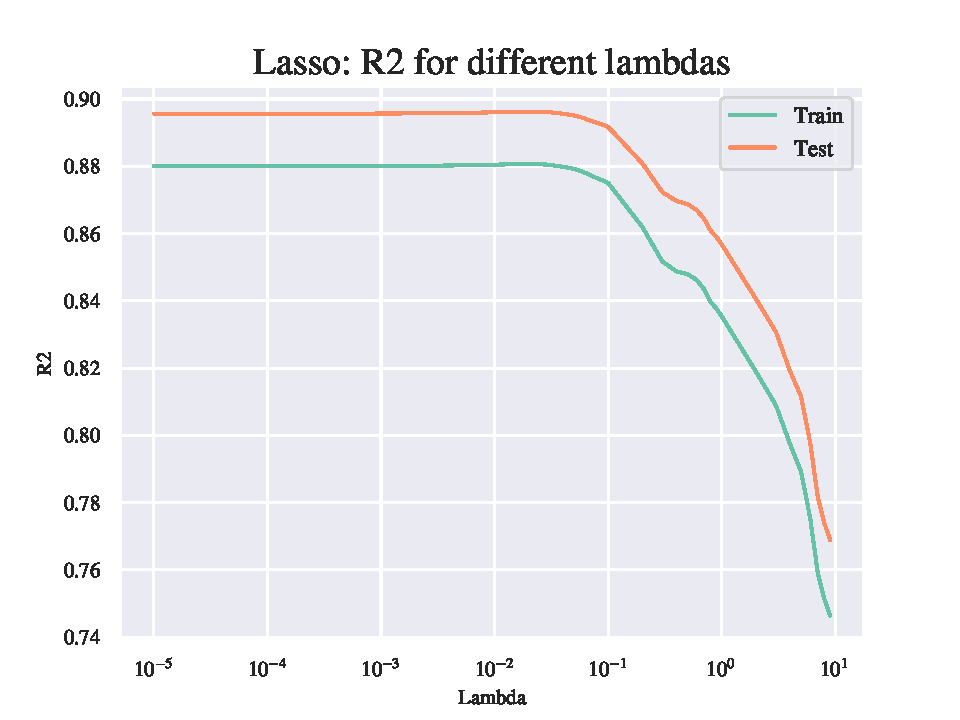
\includegraphics[width=1\linewidth]{project_1/figures/figures_in_appendix/Lasso_R2_terrain.pdf}
    \caption{Caption}
    \label{fig:ref}
\end{figure}

\begin{figure}
    \centering
    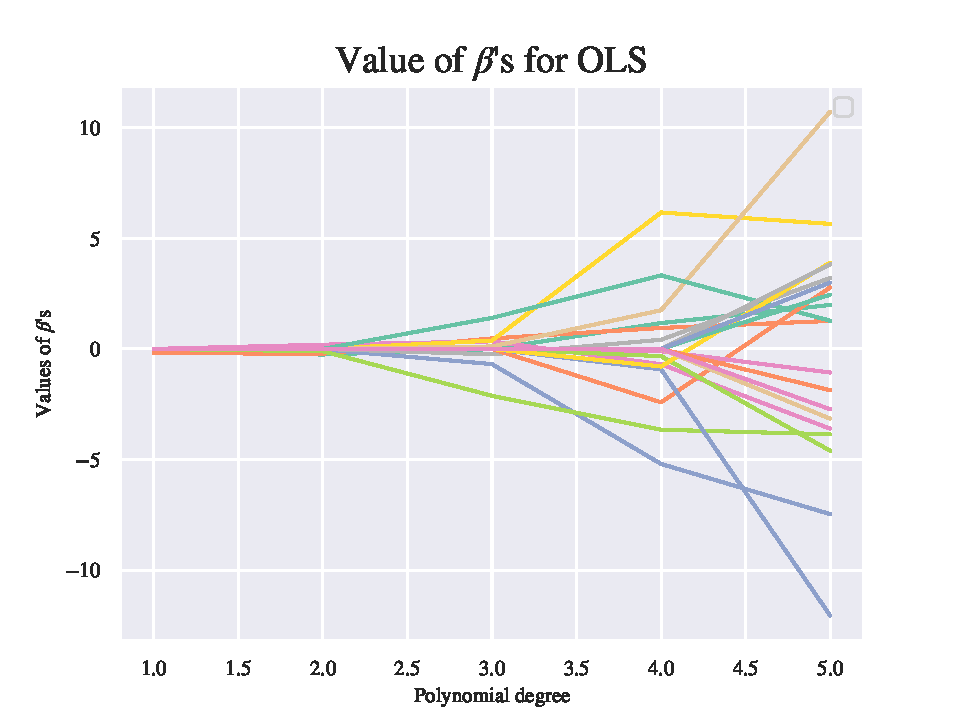
\includegraphics[width=1\linewidth]{project_1/figures/figures_in_appendix/OLS_Betas_Franke_Noise.pdf}
    \caption{Caption}
    \label{fig:ref}
\end{figure}

\begin{figure}
    \centering
    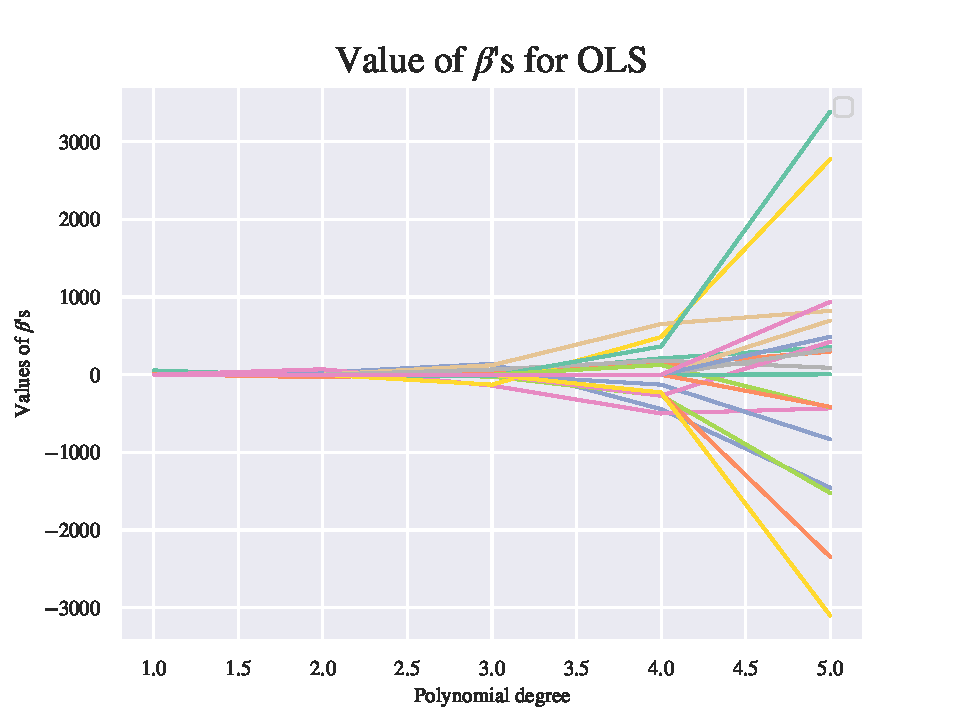
\includegraphics[width=1\linewidth]{project_1/figures/figures_in_appendix/OLS_Betas_terrain.pdf}
    \caption{Caption}
    \label{fig:ref}
\end{figure}

\begin{figure}
    \centering
    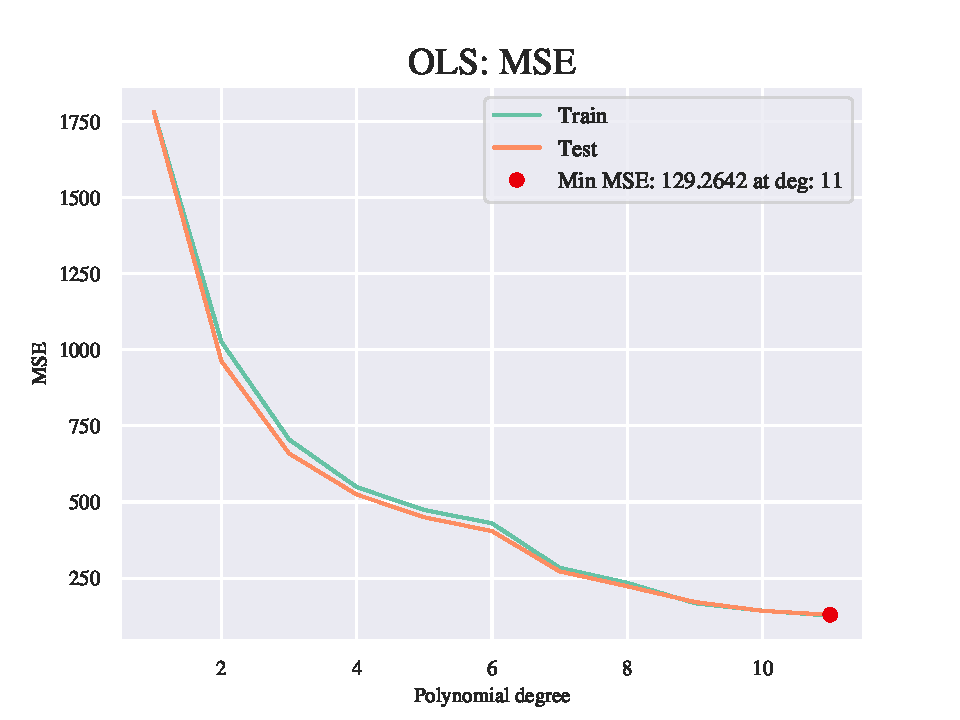
\includegraphics[width=1\linewidth]{project_1/figures/figures_in_appendix/OLS_MSE_terrain.pdf}
    \caption{Caption}
    \label{fig:ref}
\end{figure}

\begin{figure}
    \centering
    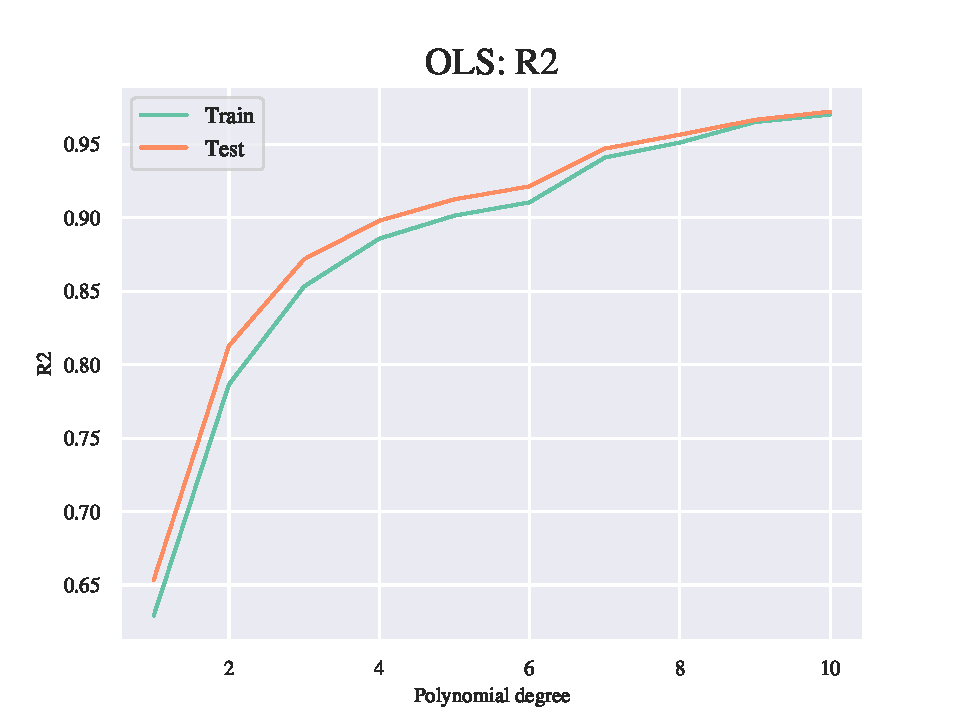
\includegraphics[width=1\linewidth]{project_1/figures/figures_in_appendix/OLS_R2_terrain.pdf}
    \caption{Caption}
    \label{fig:ref}
\end{figure}

\begin{figure}
    \centering
    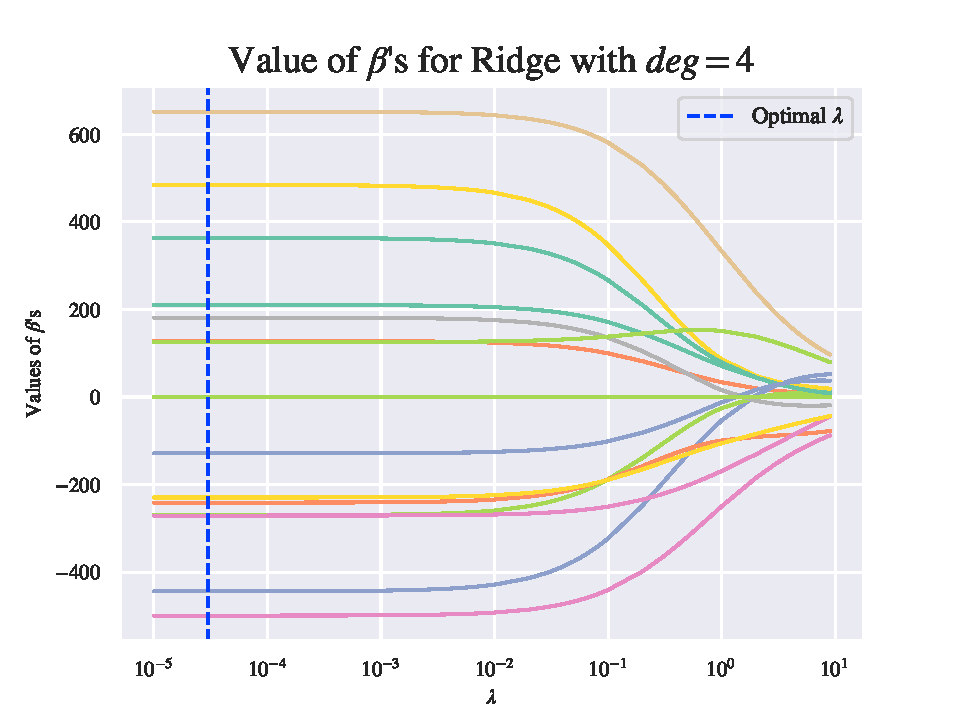
\includegraphics[width=1\linewidth]{project_1/figures/figures_in_appendix/Ridge_Betas_lambda_terrain_const_deg.pdf}
    \caption{Caption}
    \label{fig:ref}
\end{figure}

\begin{figure}
    \centering
    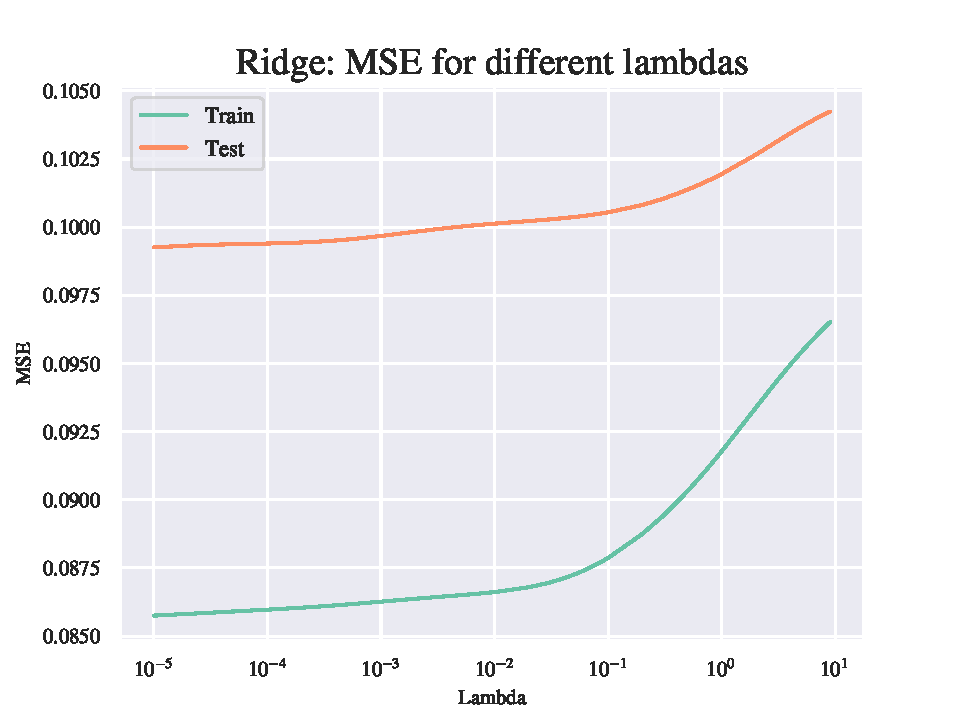
\includegraphics[width=1\linewidth]{project_1/figures/figures_in_appendix/Ridge_MSE_Franke_Noise.pdf}
    \caption{Caption}
    \label{fig:ref}
\end{figure}

\begin{figure}
    \centering
    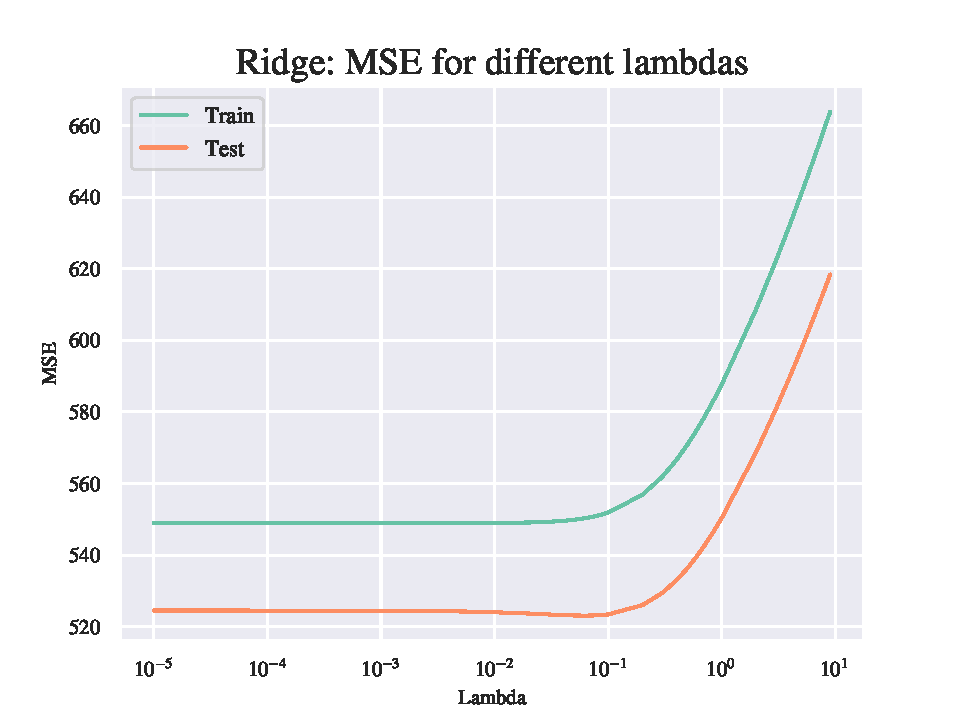
\includegraphics[width=1\linewidth]{project_1/figures/figures_in_appendix/Ridge_MSE_terrain.pdf}
    \caption{Caption}
    \label{fig:ref}
\end{figure}

\begin{figure}
    \centering
    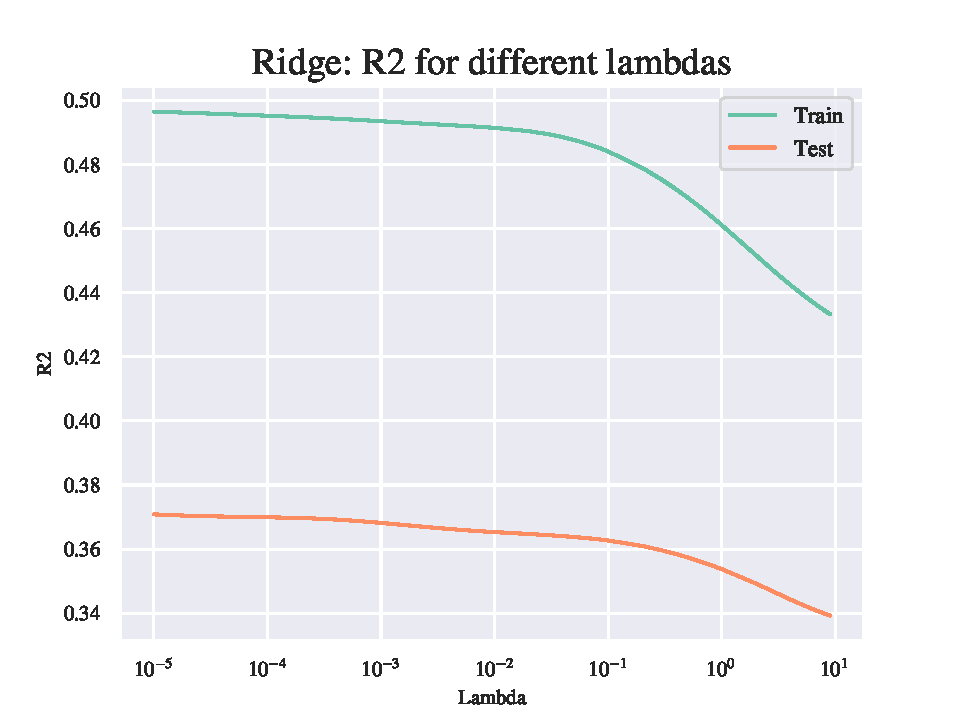
\includegraphics[width=1\linewidth]{project_1/figures/figures_in_appendix/Ridge_R2_Franke_Noise.pdf}
    \caption{Caption}
    \label{fig:ref}
\end{figure}

\begin{figure}
    \centering
    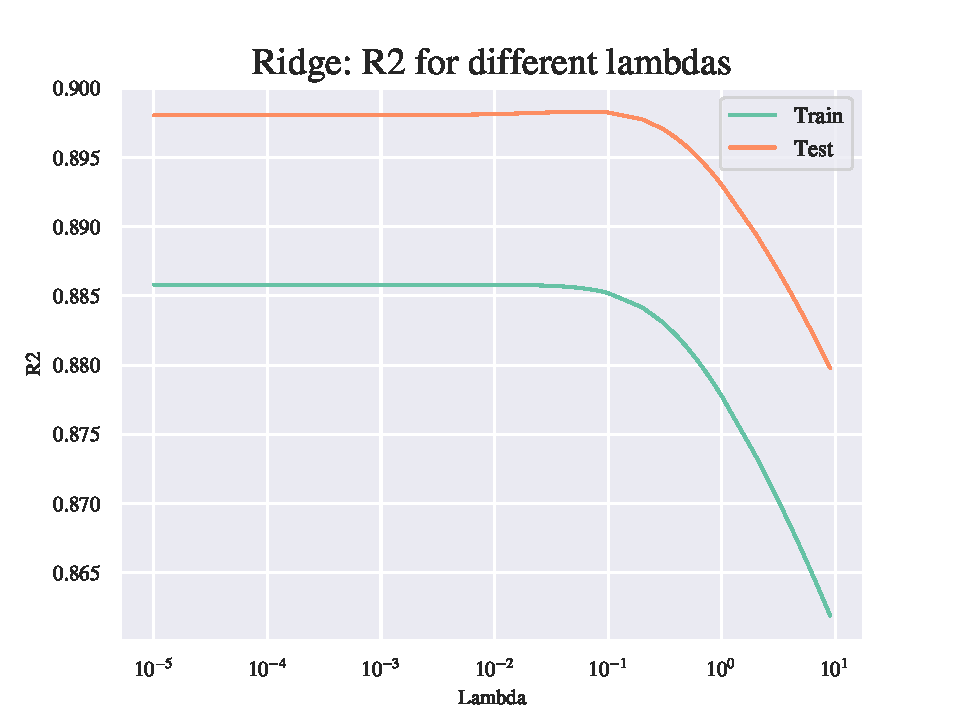
\includegraphics[width=1\linewidth]{project_1/figures/figures_in_appendix/Ridge_R2_terrain.pdf}
    \caption{Caption}
    \label{fig:ref}
\end{figure}